\documentclass{standalone}
\usepackage{tikz}
\usepackage{ctex,siunitx}
\setCJKmainfont{Noto Serif CJK SC}
\usepackage{tkz-euclide}
\usepackage{amsmath}
\usetikzlibrary{patterns, calc,3d}
\usetikzlibrary {decorations.pathmorphing,decorations.pathreplacing,decorations.shapes}
\tikzset{label style/.append style={font=\small}}
\begin{document}
\small
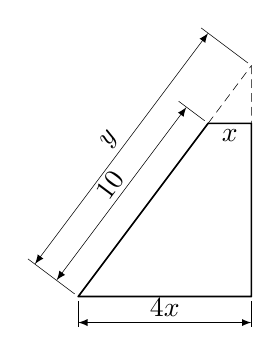
\begin{tikzpicture}[>=latex,scale=0.55,inner sep=2pt]
  \tkzDefPoints{0/0/A,4/0/B,4/4/C,3/4/D,-0.5/0.375/F,-1/0.75/G}
  \tkzInterLL(A,D)(B,C)\tkzGetPoint{E}
  \tkzDefPointsBy[translation=from A to F](D){M}
  \tkzDefPointsBy[translation=from A to G](E){N}
  \tkzDrawPolygon[semithick](A,B,C,D)
  \tkzDrawSegments[densely dashed](D,E E,C)
  \tkzLabelLine[pos=0.5,below](C,D){$x$}
  \draw[very thin,<->](0,-0.6)--(4,-0.6)node[midway,above]{$4x$};
  \draw[very thin](0,-0.1)--(0,-0.7)(4,-0.1)--(4,-0.7);
  \draw[very thin,<->](G)--(N)node[midway,sloped,above]{$y$};
  \draw[very thin,<->](F)--(M)node[midway,sloped,above]{10};
  \draw[very thin]([xshift=-0.8mm,yshift=0.6mm]D)--++(-0.6,0.45);
  \draw[very thin]([xshift=-0.8mm,yshift=0.6mm]E)--++(-1.08,0.81);
  \draw[very thin]([xshift=-0.8mm,yshift=0.6mm]A)--++(-1.08,0.81);
  % \draw[semithick](0,0)--(4,0)--(4,4)--(3,4)
\end{tikzpicture}
\end{document}